\documentclass[letterpaper]{article}
%%%%%%%%%%%%%%%%%%%%%%%%%%%%%%%%%%%%%%%%%%%%%%%%%%%%%%%%%%%%%%%%%%%%%%%%%%%%%%%%%%%%%%%%
\usepackage{makeidx}
\usepackage{natbib}
\usepackage{graphicx}
\usepackage{multicol}
\usepackage{float}
\usepackage{listings}
\usepackage{color}
\usepackage{ifthen}
\usepackage[table]{xcolor}
\usepackage{textcomp}
\usepackage{alltt}
\usepackage{ifpdf}
\ifpdf
\usepackage[pdftex,
            pagebackref=true,
            colorlinks=true,
            linkcolor=blue,
            unicode
           ]{hyperref}
\else
\usepackage[ps2pdf,
            pagebackref=true,
            colorlinks=true,
            linkcolor=blue,
            unicode
           ]{hyperref}
\usepackage{pspicture}
\fi
\usepackage{mathptmx}
\usepackage{courier}
\usepackage{sectsty}
\usepackage[titles]{tocloft}
%\usepackage{doxygen}


%%%%%%%%%%%%%%%%%%%%%%%%%%%%%%%%%%%%%%%%%%%%%%%%%%%%%%%%%%%%%%%%%%%%%%%%%%%%%%%%%%%%%%%%
\usepackage[utf8]{inputenc}
\usepackage[T1]{fontenc}
\usepackage[activeacute,spanish]{babel}
\usepackage[vmargin=4cm,tmargin=3cm,hmargin=2cm,letterpaper]{geometry}%
\usepackage{helvet}
\usepackage{amsmath,amsfonts,amssymb}
\usepackage{graphicx}
\usepackage{color}
\usepackage{xcolor}
\usepackage{verbatim}
\usepackage{tabls}
\usepackage{lastpage}
\usepackage{fancyhdr}
\usepackage{url}
\usepackage{listings}
%%%%%%%%%%%%%%%%%%%%%%%%%%%%%%%%%%%%%%%%%%%%%%%%%%%%%%%%%%%%%%%%%%%%%%%%%%%%%%%%%%%%%%%
\usepackage{tikz}
\usepackage{pgf}
\usepackage{pgffor}
\usepgfmodule{plot}
\usepackage{wrapfig}
\usetikzlibrary{arrows,decorations,snakes,backgrounds,fit,calc,through,scopes,positioning,automata,chains,er,fadings,calendar,matrix,mindmap,folding,patterns,petri,plothandlers,plotmarks,shadows,shapes,shapes.arrows,topaths,trees}

\lstset{% general command to set parameter(s)
%   basicstyle=\small,
  % print whole listing small
%   keywordstyle=\color{black}\bfseries\underbar,
  % underlined bold black keywords
%   identifierstyle=,
  % nothing happens
%   commentstyle=\color{white}, % white comments
%   stringstyle=\ttfamily,
  % typewriter type for strings
  showstringspaces=false}
  % no special string spaces

\pagestyle{fancy}
\color{black}
\fancyhead{}
\renewcommand{\headrule}{\hrule\vspace*{0.5mm}\rule{\linewidth}{0.8mm}}
\renewcommand{\familydefault}{\sfdefault}

\graphicspath{{./images/}}
\lhead{
\includegraphics[width=2cm]{logoucr.png}}
\rhead{
\includegraphics[width=3cm]{eie-text-gray-6x3cm.png}}
\chead{UNIVERSIDAD DE COSTA RICA\\FACULTAD DE INGENIERÍA\\ESCUELA DE INGENIERÍA ELÉCTRICA\\\textbf{ESTRUCTURAS ABSTRACTAS DE DATOS Y\\ ALGORITMOS PARA INGENIERÍA}\\IE-0217\\I CICLO 2014\\PROYECTO C++}

\lfoot{}%
\cfoot{}%
%\cfoot{\thepage\ de \pageref{LastPage}}%
\rfoot{}%

%%%%%%%%%%%%%%%%%%%%%%%%%%%%%%%%%%%%%%%%%%%%%%%%%%%%%%%%%%%%%%%%%%%%%%%%%%%%%%%%%%%%%%%%%%%%%%%%%%%%%%%%%%%%%%%
\newcommand{\uic}{black} %user-input color
%%%%%%%%%%%%%%%%%%%%%%%%%%%%%%%%%%%%%%%%%%%%%%%%%%%%%%%%%%%%%%%%%%%%%%%%%%%%%%%%%%%%%%%%%%%%%%%%%%%%%%%%%%%%%%%%%%
\newcommand{\uim}{} %user-input marker
%%%%%%%%%%%%%%%%%%%%%%%%%%%%%%%%%%%%%%%%%%%%%%%%%%%%%%%%%%%%%%%%%%%%%%%%%%%%%%%%%%%%%%%%%%%%%%%%%%%%%%%%%%%%%%%%%%
\newcommand{\userinput}[1]{\textcolor{\uic}{\uim#1\uim}}


%%%%%%%%%%%%%%%%%%%%%%%%%%%%%%%%%%%%%%%%%%%%%%%%%%%%%%%%%%%%%%%%%%%%%%%%%%%%%%%%%%%%%%%%%%%%%%%%%%%%%%%%%%%%%%%%%%
\begin{document}\vspace*{2cm}
%%%%%%%%%%%%%%%%%%%%%%%%%%%%%%%%%%%%%%%%%%%%%%%%%%%%%%%%%%%%%%%%%%%%%%%%%%%%%%%%%%%%%%%%%%%%%%%%%%%%%%%%%%%%%%%%%%

%%%%%%%%%%%%%%%%%%%%%%%%%%%%%%%%%%%%%%%%%%%%%%%%%%%%%%%%%%%%%%%%%%%%%%%%%%%%%%%%%%%%%%%%%%%%%%%%%%%%%%%%%%%%%%%%%%
\begin{center}
\Huge
\userinput{Body Positioning and Orientation Recognition Library KiNAO}
\vspace*{1cm}
\end{center}

\noindent
\small\baselineskip=14pt
\textbf{Estudiante:}\\
\userinput{Willy Gerardo Villalobos Marrero B17170}\\
\userinput{Daniel Méndez Zeledón            A83911}\\
\userinput{Javier Acosta Villalobos         A80056}\\


%%%%%%%%%%%%%%%%%%%%%%%%%%%%%%%%%%%%%%%%%%%%%%%%%%%%%%%%%%%%%%%%%%%%%%%%%%%%%%%%%%%%%%%%%%%%%%%%%%%%%%%%%%%%%%%%%%
\tableofcontents
\pagenumbering{arabic}
\pagebreak
\section{Introducción}

Como parte del desarrollo de reconocimiento de patrones, se ha tratado de elaborar una pequeña librería la cual permitiese tomar, a partir de una cámara de Kinect, el esqueleto de una persona, mediante un algoritmo. Luego, con las posiciones X, Y, Z de cada uno de los puntos de los ligamentos del cuerpo, se podría analizar el movimiento de cada parte del cuerpo. Debido a que la cámara del Kinect permite analizar la profundidad, es, de cierta manera, sencillo analizar las posiciones, no solamente las que se muestran en el plano XY. Para este análisis, se utilizará como base la librería OpenNI que permite controlar, de manera eficaz, la cámara del Kinect, así como obtener los parámetros que el Kinect analiza.\\

Ya con los valores XYZ asignados, se logra obtener los ángulos de los ligamentos del cuerpo en tiempo real a partir de la ley de cosenos, donde con 2 partes del cuerpo y una línea imaginaria, se logra determinar el ángulo respectivo para el ligamento y así obtener su valor.\\

		\begin{figure}[h!]
			\centering
			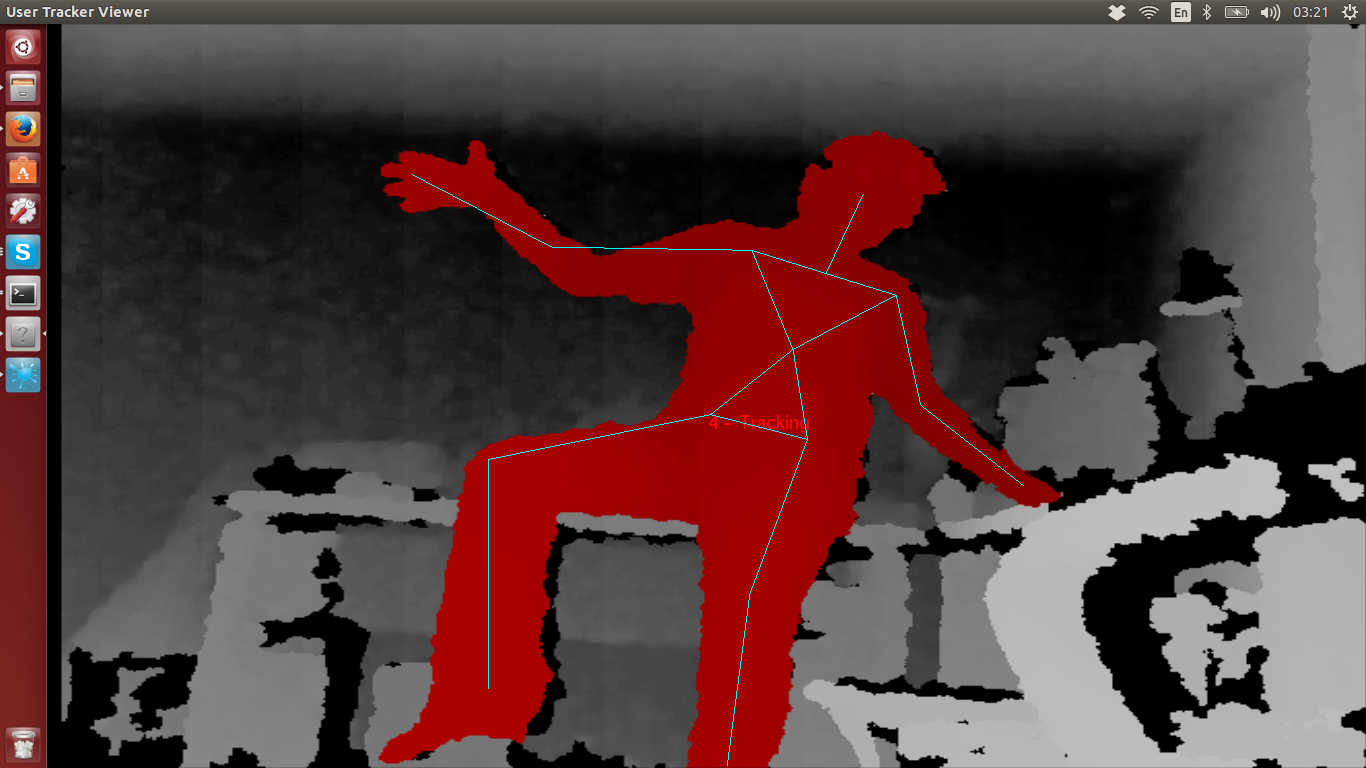
\includegraphics[width=0.7\linewidth]{imagenes/person.png}
			\caption{Imagen de esqueleto virtual generado mediante OpenNi}
		\end{figure}

La razón de nuestro proyecto cabe en el ámbito de las teleoperaciones. Como un nuevo paso hacia este tema, se quiere poder hacer en movimientos en tiempo real de tal forma que puedan ser transferidos a un robot y este haga trabajos en zonas de alto riesgo, por ejemplo en un edificio después de un terremoto, en el espacio, en alguna planta nuclear, donde, a pesar del precio que se paga por cada robot, no importe si se daña, pues no se estará arriesgando vidas humanas en el intento de los distintos trabajos de alto riesgo.\\

		\begin{figure}[h!]
			\centering
			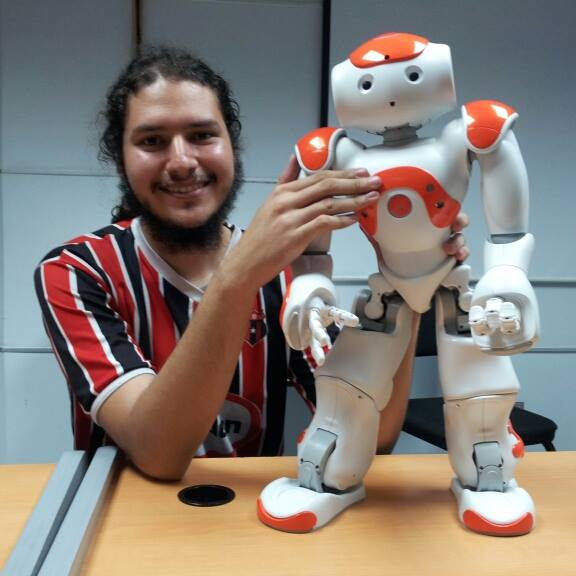
\includegraphics[width=0.4\linewidth]{imagenes/nao_and_me.jpg}
			\caption{Fotografía de robot NAO con estudiante}
		\end{figure}

Es por eso que la librería va orientada a esto, usar los ángulos de los ligamentos para ser traspasados a los robots que actualmente se encuentran en disposicion de la Escuela de Ingeniería Eléctrica, los NAO, donde los parámetros se le pueden pasar a través de ángulos en radianes y el robot podrá imitar los movimientos que se estén haciendo en tiempo real frente a la cámara del Kinect.\\

%%%%%%%%%%%%%%%%%%%%%%%%%%%%%%%%%%%%%%%%%%%%%%%%%%%%%%%%%%%%%%%%%%%%%%%%%%%%%%%%%%%%%%%%%%%%%%%%%%%%%%%%%%%%%%%%%%
\section{Objetivos}
\subsection{Objetivo General}

Crear una librería capaz de reconocer los movimientos de cuerpo entero a travéz de la cámara Kinect, utilizando la librería de OpenNI como base del desarrollo, con el fin de hacer que los robots NAO traten de imitar estos movimientos a partir de los parámetros determinados por la librería.

\subsection{Objetivos Específicos}

\begin{itemize}
\item Crear una librería que controle el movimiento por separado de la cabeza, brazos, manos, piernas y pies, utilizando el lenguaje de programación C++, con el fin de ejercer clases para utilizar el lenguaje orientado a objetos.
\item Utilizar la ley de cosenos como base para la obtención de los ángulos de los ligamentos del cuerpo, tomando como referencia los puntos identificados por el algoritmo de identificación de ligamentos que incluye la libreria OpenNI.
\item Crear unas funciones para trasladar los ángulos obtenidos a los NAO para tratar de hacer que éstos se muevan en tiempo real con el movimientos que esté analizando el Kinect.
\end{itemize}

\section{Funciones agregadas}

Entre las operaciones básicas de álgebra lineal que se consideraron necesarias para la implementación del KiNAO están las operaciones de producto punto y producto vectorial, identidades relacionadas con ángulos entre vectores ($\cos{\Theta}, \sen{\Theta}$), módulo de un vector, proyecciones, etc. Dichas funciones fueron agregadas al archivo "joint.cpp" y son las que se emplean para, inicialmente, generar vectores a partir de los joints, definidos cada uno como un punto con coordenadas $(X,Y,Z)$.\\ 

Posterior a la obtención de dichos vectores, se realizan operaciones de producto vectorial para obtener el vector ortogonal, el cual, sumado a la obtención de proyecciones de vectores sobre uns superficie hipotética, nos permite obtener los ángulos de roll, pitch y yaw de la extremidad. Dicha información es posteriormente transformada en valores compatibles con el autómata,  en este caso un NAO.\\

La idea básicamente es generar planos sobre los cuales los brazos se van a mover, de forma que sea posible entonces detectar variaciones en la rotación de las extremidades.\\

A la hora de trasladar la información de ángulos a un robot, se debe tener en cuenta que, por ejemplo, lo que se  puede extender un brazo humano en grados, no es lo mismo que lo que se puede extender un NAO, por lo que se debe tener en consideración ese hecho. En este caso se plantea un condicional para que en caso de que el ángulo de rotación de una extremidad humana supere la máxima extensión del robot, simplemente se sigue restringiendo la información de manera que el automata nunca extienda sus extremidades más allá de lo que puede hacerlo físicamente.\\

Un próximo paso será plantear una escala de variación de manera que no solo se consideren los valores extremos de extensión del robot, sino que se pueda realizar una calibración con la persona para que los movimientos del humano sean realizados por el robot siguiendo una escala adecuada para que la máxima extensión del humano coincida con la del robot.\\

Cabe resaltar que el despliegue de información, empezando por el esqueleto, se realiza tomando como base el generador de esqueletos de OpenNI.\\

%%%%%%%%%%%%%%%%%%%%%%%%%%%%%%%%%%%%%%%%%%%%%%%%%%%%%%%%%%%%%%%%%%%%%%%%%%%%%%%%%%%%%%%%%%%%%%%%%%%%%%%%%%%%%%%%%%

\hypertarget{class_joint}{\section{Joint Class Reference}
\label{class_joint}\index{Joint@{Joint}}
}


Aqui se describe la clase base \char`\"{}\-Joint\char`\"{}.  




{\ttfamily \#include $<$joint.\-h$>$}

Inheritance diagram for Joint\-:\begin{figure}[H]
\begin{center}
\leavevmode
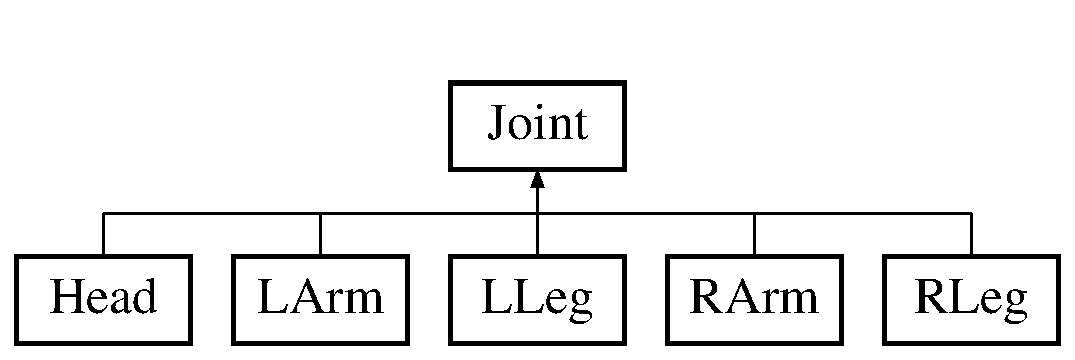
\includegraphics[height=2.000000cm]{class_joint}
\end{center}
\end{figure}
\subsection*{Public Member Functions}
\begin{DoxyCompactItemize}
\item 
\hypertarget{class_joint_a79a7a4715b2166714e039d7c7c5ea3b4}{\hyperlink{class_joint_a79a7a4715b2166714e039d7c7c5ea3b4}{Joint} ()}\label{class_joint_a79a7a4715b2166714e039d7c7c5ea3b4}

\begin{DoxyCompactList}\small\item\em Esta es la decralarion de la funcionalidad de la clase base \char`\"{}\-Joint\char`\"{}, de aqui se deriban las demas. \end{DoxyCompactList}\item 
\hypertarget{class_joint_ac9749eeeac49e9861554f2d580cc020d}{virtual \hyperlink{class_joint_ac9749eeeac49e9861554f2d580cc020d}{$\sim$\-Joint} (void)}\label{class_joint_ac9749eeeac49e9861554f2d580cc020d}

\begin{DoxyCompactList}\small\item\em Constructor del Objeto. \end{DoxyCompactList}\item 
virtual float \hyperlink{class_joint_a1b4c78e285a1d96bbde889d4979828fa}{length} (float\mbox{[}3\mbox{]}, float\mbox{[}3\mbox{]})
\begin{DoxyCompactList}\small\item\em Destructor del Objeto. \end{DoxyCompactList}\item 
virtual float \hyperlink{class_joint_ab4a853045a69e77e8b67d195be145eed}{angle} (float, float, float)
\item 
virtual float \hyperlink{class_joint_a52f2f6003f4cff059847d959488622a1}{get\-Angle} (Xn\-Vector3\-D, Xn\-Vector3\-D, Xn\-Vector3\-D)
\begin{DoxyCompactList}\small\item\em L1,L2,L3(\-L3 es el opuesto del angulo a determinar) \end{DoxyCompactList}\item 
virtual Xn\-Vector3\-D \hyperlink{class_joint_ac59f570adbaf039bbe0f4173e5e7e2ce}{get\-Normal\-Vector} (Xn\-Vector3\-D, Xn\-Vector3\-D, Xn\-Vector3\-D)
\begin{DoxyCompactList}\small\item\em Genera el vector resultante de realizar el producto cruz entre los 2 vectores coplanares. \end{DoxyCompactList}\item 
virtual Xn\-Vector3\-D \hyperlink{class_joint_af5590ba3d5bfc4e27a43036a1d394629}{get\-Proyection\-Vector} (Xn\-Vector3\-D, Xn\-Vector3\-D)
\begin{DoxyCompactList}\small\item\em Obtiene el vector resultante de proyectar un vector sobre otro. \end{DoxyCompactList}\item 
virtual Xn\-Float \hyperlink{class_joint_a06ed69732a17f61fa6ce9fa5ba2541ea}{get\-Proyection} (Xn\-Vector3\-D Vector1, Xn\-Vector3\-D Vector2)
\begin{DoxyCompactList}\small\item\em Obtiene la constante de la proyeccion. \end{DoxyCompactList}\item 
virtual \hyperlink{struct_xn_reference_axis}{Xn\-Reference\-Axis} \hyperlink{class_joint_a603eab4701f005bc6a39911897eb6c7d}{generate\-Reference} (Xn\-Vector3\-D, Xn\-Vector3\-D, Xn\-Vector3\-D)
\begin{DoxyCompactList}\small\item\em Construye un nuevo eje de coordenadas a partir de 3 vectores otrtogonales. \end{DoxyCompactList}\end{DoxyCompactItemize}


\subsection{Detailed Description}
Aqui se describe la clase base \char`\"{}\-Joint\char`\"{}. 

\subsection{Member Function Documentation}
\hypertarget{class_joint_ab4a853045a69e77e8b67d195be145eed}{\index{Joint@{Joint}!angle@{angle}}
\index{angle@{angle}!Joint@{Joint}}
\subsubsection[{angle}]{\setlength{\rightskip}{0pt plus 5cm}float Joint\-::angle (
\begin{DoxyParamCaption}
\item[{float}]{R\-L1, }
\item[{float}]{R\-L2, }
\item[{float}]{I\-M\-L3}
\end{DoxyParamCaption}
)\hspace{0.3cm}{\ttfamily [virtual]}}}\label{class_joint_ab4a853045a69e77e8b67d195be145eed}
P1\mbox{[}3\mbox{]},P2\mbox{[}3\mbox{]} Determina el angulo entre 3 puntos dadas las 3 lineas descritas por estos puntos El angulo a determinar viene dado por la linea imaginaria que esta opuesta a este angulo I\-M\-L3 es el segmento contrario al angulo por determinar, el cual no existe, es I\-Maginario \hypertarget{class_joint_a603eab4701f005bc6a39911897eb6c7d}{\index{Joint@{Joint}!generate\-Reference@{generate\-Reference}}
\index{generate\-Reference@{generate\-Reference}!Joint@{Joint}}
\subsubsection[{generate\-Reference}]{\setlength{\rightskip}{0pt plus 5cm}{\bf Xn\-Reference\-Axis} Joint\-::generate\-Reference (
\begin{DoxyParamCaption}
\item[{Xn\-Vector3\-D}]{J1, }
\item[{Xn\-Vector3\-D}]{J2, }
\item[{Xn\-Vector3\-D}]{J3}
\end{DoxyParamCaption}
)\hspace{0.3cm}{\ttfamily [virtual]}}}\label{class_joint_a603eab4701f005bc6a39911897eb6c7d}


Construye un nuevo eje de coordenadas a partir de 3 vectores otrtogonales. 

Este método genera un nuevo eje de referencia centrado en un \hyperlink{class_joint}{Joint}. Point\-Normal1 es un nuevo \hyperlink{class_joint}{Joint} para calcular una de las normales que será parte del marco de referencia

Utilizamos el struct \hyperlink{struct_xn_reference_axis}{Xn\-Reference\-Axis} definido previamente para almacenar el nuevo marco de referencia \hypertarget{class_joint_a52f2f6003f4cff059847d959488622a1}{\index{Joint@{Joint}!get\-Angle@{get\-Angle}}
\index{get\-Angle@{get\-Angle}!Joint@{Joint}}
\subsubsection[{get\-Angle}]{\setlength{\rightskip}{0pt plus 5cm}float Joint\-::get\-Angle (
\begin{DoxyParamCaption}
\item[{Xn\-Vector3\-D}]{J1, }
\item[{Xn\-Vector3\-D}]{J2, }
\item[{Xn\-Vector3\-D}]{J3}
\end{DoxyParamCaption}
)\hspace{0.3cm}{\ttfamily [virtual]}}}\label{class_joint_a52f2f6003f4cff059847d959488622a1}


L1,L2,L3(\-L3 es el opuesto del angulo a determinar) 

J2 es la articulacion a la que se va a sacar el angulo.

Aunque se podria, no se crea una funcion get\-Angle aqui porque se necesitan pasar los parametros que usa el kinect para cada una de las posiciones, lo que se quiere es simplemente decir head.\-get\-Angle y que se obtenga el de la cabeza. Se pordria hacer, pero inicializando todos los joints y que se esten actualizando en tiempo real en la clasd \hyperlink{class_joint}{Joint}, para luego simplemente llamarlos desde las respectivas subclases igualando el valor actual del \hyperlink{class_joint}{Joint} en x,y,z a mi variable dentro de la subclase, luego como el objeto es de tipo \hyperlink{class_head}{Head}, entonces el automaticamente sabe que las variables que debe pasar son las corerspondientes a los puntos que describen el angulo del cuello. Por ahora queda como mejora Determina directamente el angulo que hay en el segundo vector Se toman los tres vectores y se determina la distancia entre ellos, donde Imag3 es la distancia opuesta el J2 \hypertarget{class_joint_ac59f570adbaf039bbe0f4173e5e7e2ce}{\index{Joint@{Joint}!get\-Normal\-Vector@{get\-Normal\-Vector}}
\index{get\-Normal\-Vector@{get\-Normal\-Vector}!Joint@{Joint}}
\subsubsection[{get\-Normal\-Vector}]{\setlength{\rightskip}{0pt plus 5cm}Xn\-Vector3\-D Joint\-::get\-Normal\-Vector (
\begin{DoxyParamCaption}
\item[{Xn\-Vector3\-D}]{J1, }
\item[{Xn\-Vector3\-D}]{J2, }
\item[{Xn\-Vector3\-D}]{J3}
\end{DoxyParamCaption}
)\hspace{0.3cm}{\ttfamily [virtual]}}}\label{class_joint_ac59f570adbaf039bbe0f4173e5e7e2ce}


Genera el vector resultante de realizar el producto cruz entre los 2 vectores coplanares. 

J2 es el punto de unión de los vectores J2-\/$>$J1 y J2-\/$>$J3, a los cuales se les sacará el vector normal. Generamos 2 vectores a partir de los cuales calcularemos el producto cruz, Vector1 X Vector2 = Vector\-Normal

Para Vector1 = J2-\/$>$J1

Para Vector2 = J2-\/$>$J3

Generamos el vector ortogonal Vector\-Normal \hypertarget{class_joint_a06ed69732a17f61fa6ce9fa5ba2541ea}{\index{Joint@{Joint}!get\-Proyection@{get\-Proyection}}
\index{get\-Proyection@{get\-Proyection}!Joint@{Joint}}
\subsubsection[{get\-Proyection}]{\setlength{\rightskip}{0pt plus 5cm}Xn\-Float Joint\-::get\-Proyection (
\begin{DoxyParamCaption}
\item[{Xn\-Vector3\-D}]{Vector1, }
\item[{Xn\-Vector3\-D}]{Vector2}
\end{DoxyParamCaption}
)\hspace{0.3cm}{\ttfamily [virtual]}}}\label{class_joint_a06ed69732a17f61fa6ce9fa5ba2541ea}


Obtiene la constante de la proyeccion. 

Calculamos la proyección del Vector1 sobre el Vector2. Generamos el vector en el cual se va a guardar la proyección resultante

Calculamos el producto punto entre Vector1 y Vector2

Calculamos la norma del Vector2

Ahora calculamos la constante que multiplica al vector sobre el cual estamos proyectando para generar el nuevo vector proyección \hypertarget{class_joint_af5590ba3d5bfc4e27a43036a1d394629}{\index{Joint@{Joint}!get\-Proyection\-Vector@{get\-Proyection\-Vector}}
\index{get\-Proyection\-Vector@{get\-Proyection\-Vector}!Joint@{Joint}}
\subsubsection[{get\-Proyection\-Vector}]{\setlength{\rightskip}{0pt plus 5cm}Xn\-Vector3\-D Joint\-::get\-Proyection\-Vector (
\begin{DoxyParamCaption}
\item[{Xn\-Vector3\-D}]{Vector1, }
\item[{Xn\-Vector3\-D}]{Vector2}
\end{DoxyParamCaption}
)\hspace{0.3cm}{\ttfamily [virtual]}}}\label{class_joint_af5590ba3d5bfc4e27a43036a1d394629}


Obtiene el vector resultante de proyectar un vector sobre otro. 

Calculamos la proyección del Vector1 sobre el Vector2. Generamos el vector en el cual se va a guardar la proyección resultante

Calculamos el producto punto entre Vector1 y Vector2

Calculamos la norma del Vector2 \hypertarget{class_joint_a1b4c78e285a1d96bbde889d4979828fa}{\index{Joint@{Joint}!length@{length}}
\index{length@{length}!Joint@{Joint}}
\subsubsection[{length}]{\setlength{\rightskip}{0pt plus 5cm}float Joint\-::length (
\begin{DoxyParamCaption}
\item[{float}]{p1\mbox{[}3\mbox{]}, }
\item[{float}]{p2\mbox{[}3\mbox{]}}
\end{DoxyParamCaption}
)\hspace{0.3cm}{\ttfamily [virtual]}}}\label{class_joint_a1b4c78e285a1d96bbde889d4979828fa}


Destructor del Objeto. 

Determina el vector que va de P1 a P2 Determina el vector que va de P1 a P2 

The documentation for this class was generated from the following files\-:\begin{DoxyCompactItemize}
\item 
/home/daniel/\-U\-C\-R/\-Ey\-A\-Team/kinect/\-Open\-N\-I\-\_\-\-N\-I\-T\-E\-\_\-\-Installer-\/\-Linux64-\/0.\-27/\-Open\-N\-I-\/\-Bin-\/\-Dev-\/\-Linux-\/x64-\/v1.\-5.\-4.\-0/\-Samples/\-Ni\-Simple\-Skeleton/kinao/joint.\-h\item 
/home/daniel/\-U\-C\-R/\-Ey\-A\-Team/kinect/\-Open\-N\-I\-\_\-\-N\-I\-T\-E\-\_\-\-Installer-\/\-Linux64-\/0.\-27/\-Open\-N\-I-\/\-Bin-\/\-Dev-\/\-Linux-\/x64-\/v1.\-5.\-4.\-0/\-Samples/\-Ni\-Simple\-Skeleton/kinao/joint.\-cpp\item 
/home/daniel/\-U\-C\-R/\-Ey\-A\-Team/kinect/\-Open\-N\-I\-\_\-\-N\-I\-T\-E\-\_\-\-Installer-\/\-Linux64-\/0.\-27/\-Open\-N\-I-\/\-Bin-\/\-Dev-\/\-Linux-\/x64-\/v1.\-5.\-4.\-0/\-Samples/\-Ni\-Simple\-Skeleton/kinao/normal.\-cpp\end{DoxyCompactItemize}

\hypertarget{class_head}{\section{Head Class Reference}
\label{class_head}\index{Head@{Head}}
}


Aqui se describe la clase derivada \char`\"{}\-Head\char`\"{}.  




{\ttfamily \#include $<$joint.\-h$>$}

Inheritance diagram for Head\-:\begin{figure}[H]
\begin{center}
\leavevmode
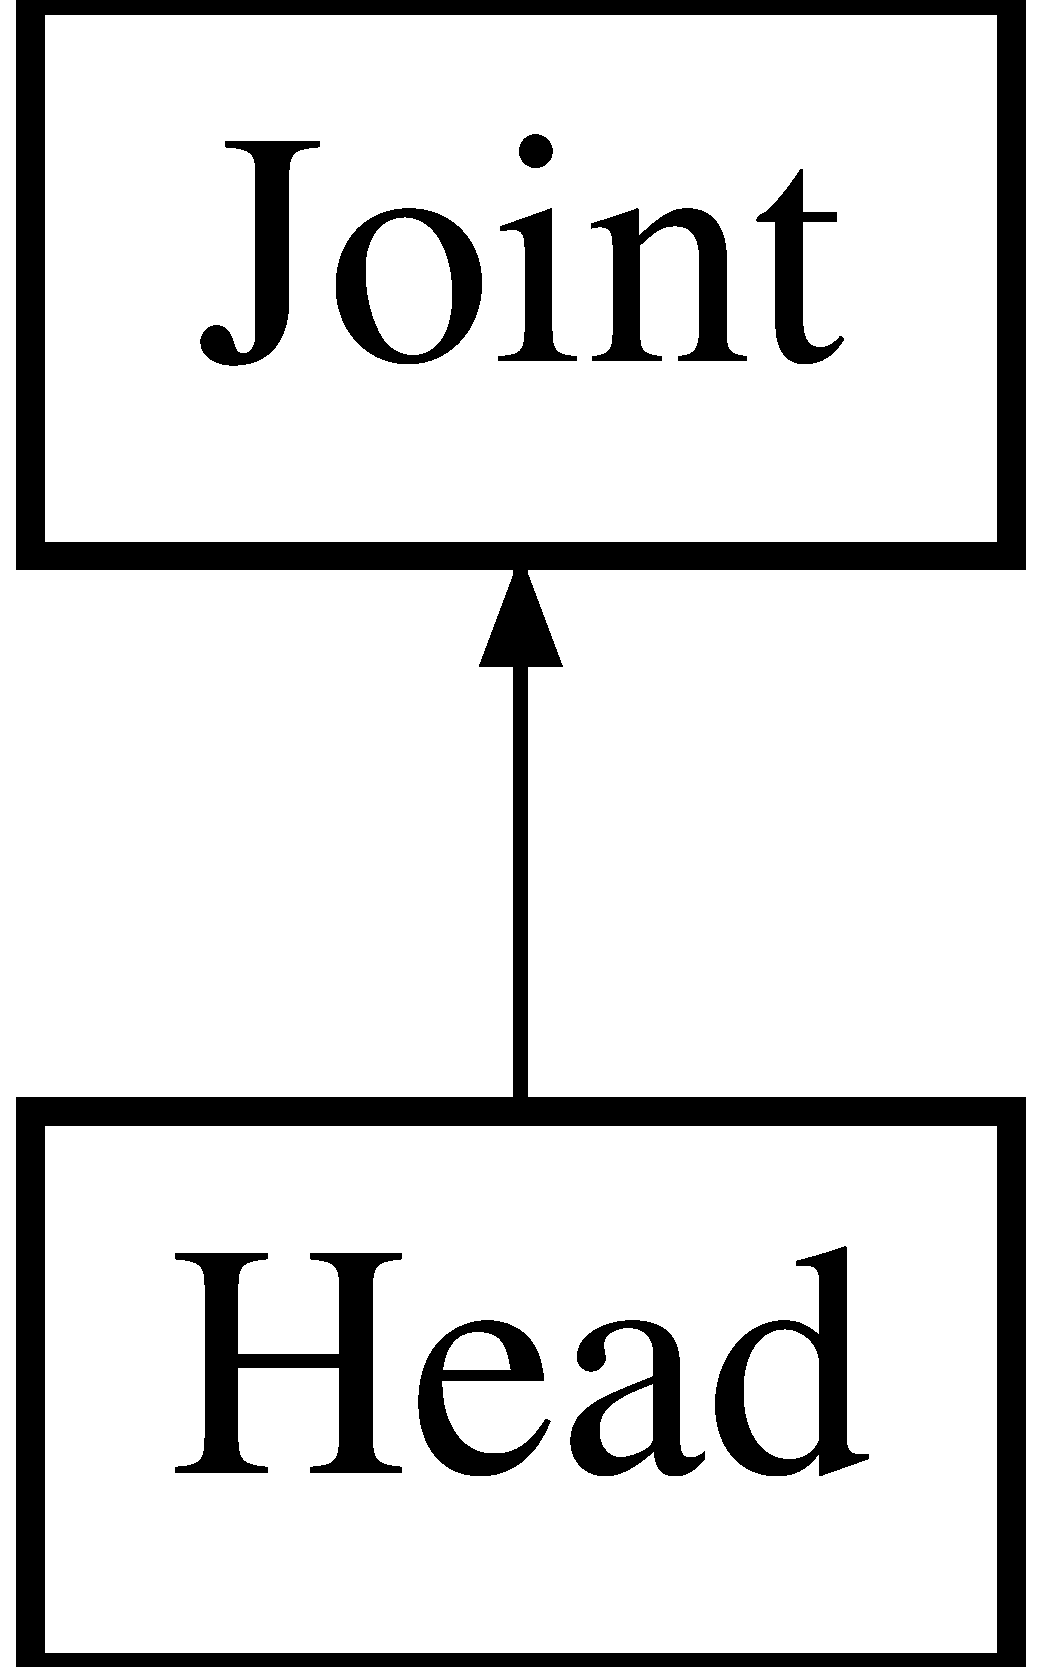
\includegraphics[height=2.000000cm]{class_head}
\end{center}
\end{figure}
\subsection*{Public Member Functions}
\begin{DoxyCompactItemize}
\item 
\hypertarget{class_head_a0a4e931e188a25b60f6b992ff32f7bfa}{\hyperlink{class_head_a0a4e931e188a25b60f6b992ff32f7bfa}{Head} ()}\label{class_head_a0a4e931e188a25b60f6b992ff32f7bfa}

\begin{DoxyCompactList}\small\item\em Declaracion de la clase derivada \char`\"{}\-Head\char`\"{} y su funcionalidad. \end{DoxyCompactList}\item 
\hypertarget{class_head_a502987ba6c8d6b615977150dd565fc27}{virtual \hyperlink{class_head_a502987ba6c8d6b615977150dd565fc27}{$\sim$\-Head} (void)}\label{class_head_a502987ba6c8d6b615977150dd565fc27}

\begin{DoxyCompactList}\small\item\em Constructor del Objeto. \end{DoxyCompactList}\item 
virtual float \hyperlink{class_head_ad57a93c84de0a6681dce1dbcdc87823c}{get\-Head\-Pitch} (Xn\-User\-I\-D, xn\-::\-User\-Generator)
\begin{DoxyCompactList}\small\item\em Obtiene el angulo que se determina a partir del kinect. \end{DoxyCompactList}\item 
\hypertarget{class_head_a6f624a1b326a840aad5221608809f40f}{virtual float \hyperlink{class_head_a6f624a1b326a840aad5221608809f40f}{set\-Head\-Pitch} (float, float \&, float \&)}\label{class_head_a6f624a1b326a840aad5221608809f40f}

\begin{DoxyCompactList}\small\item\em Genera el angulo necesario para mover el N\-A\-O. \end{DoxyCompactList}\end{DoxyCompactItemize}


\subsection{Detailed Description}
Aqui se describe la clase derivada \char`\"{}\-Head\char`\"{}. 

\subsection{Member Function Documentation}
\hypertarget{class_head_ad57a93c84de0a6681dce1dbcdc87823c}{\index{Head@{Head}!get\-Head\-Pitch@{get\-Head\-Pitch}}
\index{get\-Head\-Pitch@{get\-Head\-Pitch}!Head@{Head}}
\subsubsection[{get\-Head\-Pitch}]{\setlength{\rightskip}{0pt plus 5cm}float Head\-::get\-Head\-Pitch (
\begin{DoxyParamCaption}
\item[{Xn\-User\-I\-D}]{user, }
\item[{xn\-::\-User\-Generator}]{guser}
\end{DoxyParamCaption}
)\hspace{0.3cm}{\ttfamily [virtual]}}}\label{class_head_ad57a93c84de0a6681dce1dbcdc87823c}


Obtiene el angulo que se determina a partir del kinect. 

Obtiene el angulo real dado por el kinect del movimiento frontal de la cabeza.

Destructor del Objeto 

The documentation for this class was generated from the following files\-:\begin{DoxyCompactItemize}
\item 
/home/daniel/\-U\-C\-R/\-Ey\-A\-Team/kinect/\-Open\-N\-I\-\_\-\-N\-I\-T\-E\-\_\-\-Installer-\/\-Linux64-\/0.\-27/\-Open\-N\-I-\/\-Bin-\/\-Dev-\/\-Linux-\/x64-\/v1.\-5.\-4.\-0/\-Samples/\-Ni\-Simple\-Skeleton/kinao/joint.\-h\item 
/home/daniel/\-U\-C\-R/\-Ey\-A\-Team/kinect/\-Open\-N\-I\-\_\-\-N\-I\-T\-E\-\_\-\-Installer-\/\-Linux64-\/0.\-27/\-Open\-N\-I-\/\-Bin-\/\-Dev-\/\-Linux-\/x64-\/v1.\-5.\-4.\-0/\-Samples/\-Ni\-Simple\-Skeleton/kinao/head.\-cpp\end{DoxyCompactItemize}

\hypertarget{class_l_arm}{\section{\-Referencia de \-Clase \-L\-Arm}
\label{class_l_arm}\index{\-L\-Arm@{\-L\-Arm}}
}


\-Esta es la clase que describe el comportamiento para el brazo izquierdo.  




{\ttfamily \#include $<$joint.\-h$>$}

\-Diagrama de herencia para \-L\-Arm\-:\begin{figure}[H]
\begin{center}
\leavevmode
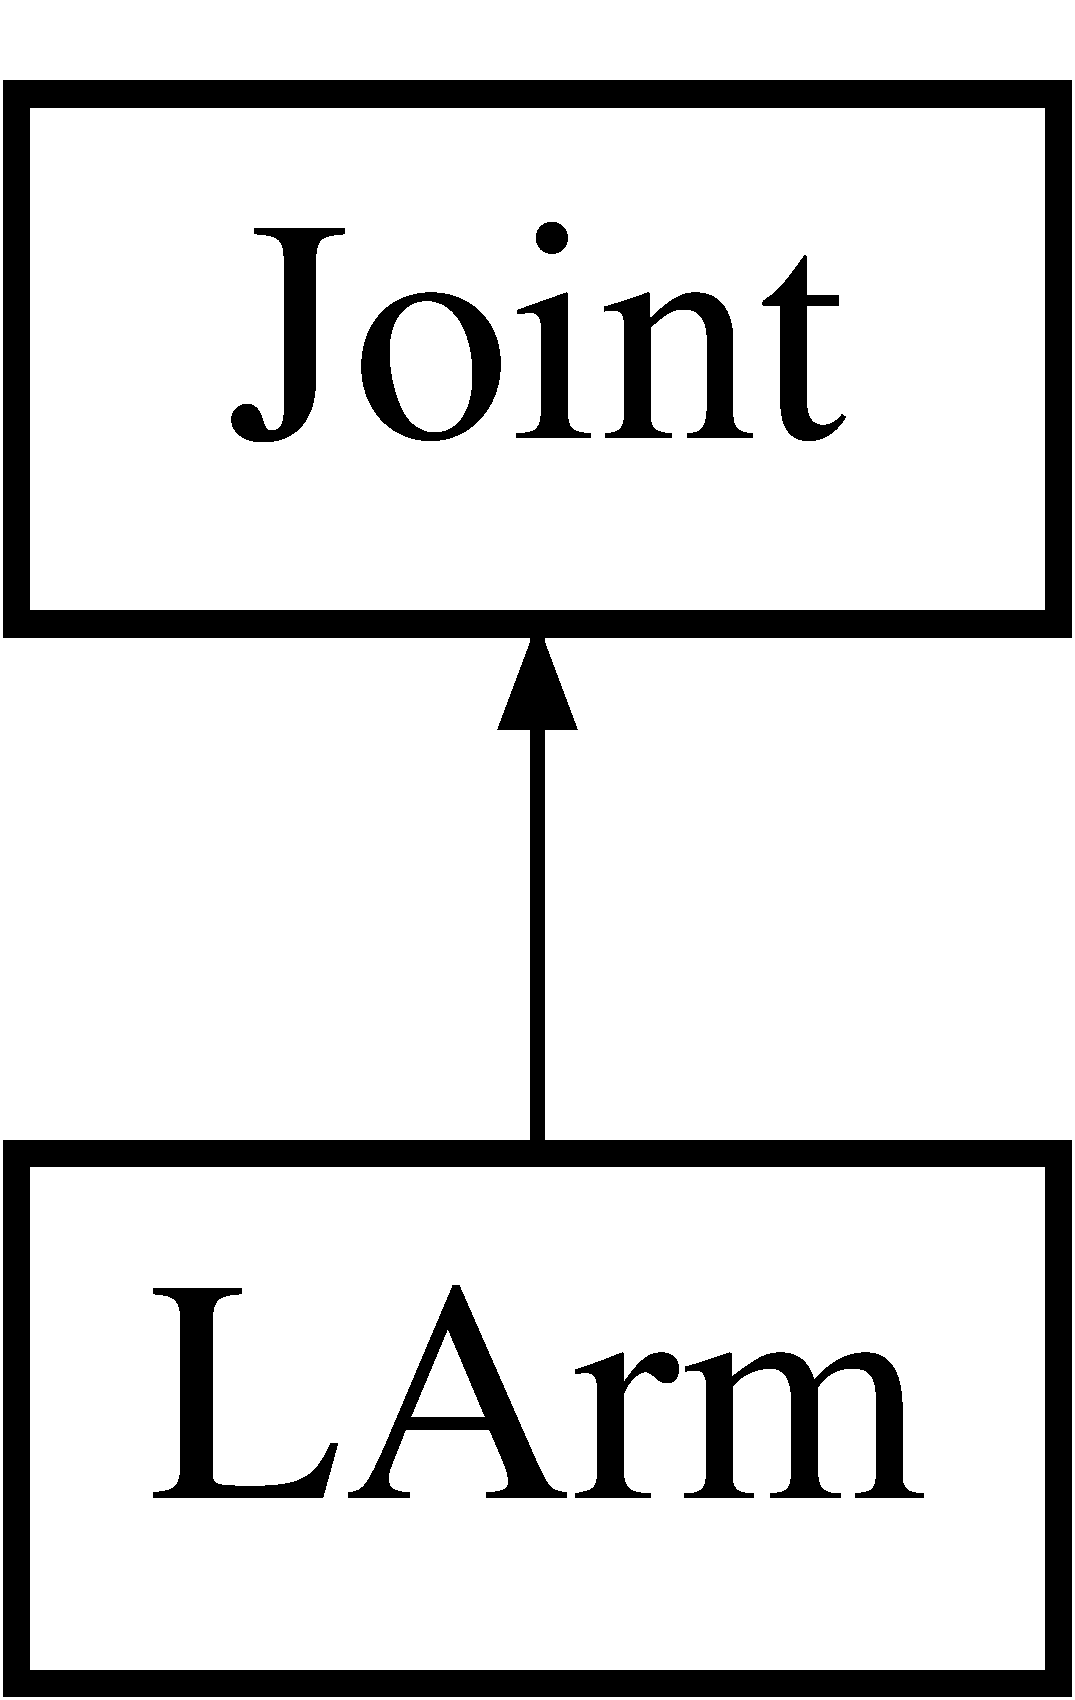
\includegraphics[height=2.000000cm]{class_l_arm}
\end{center}
\end{figure}
\subsection*{\-Funciones \-Miembro \-Públicas}
\begin{itemize}
\item 
virtual float \hyperlink{class_l_arm_aca3aa8c68dedd1c7fb1e0ed9ba55b239}{get\-Elbow\-Roll} (\-Xn\-User\-I\-D, xn\-::\-User\-Generator)
\begin{itemize}\small\item\em \-Obtiene el ángulo que se determina a partir del kinect del codo. \end{itemize}\item 
\hypertarget{class_l_arm_a19580475d6f1d5ae421a419a090f835e}{virtual float \hyperlink{class_l_arm_a19580475d6f1d5ae421a419a090f835e}{set\-Elbow\-Roll} (float, float \&, float \&)}\label{class_l_arm_a19580475d6f1d5ae421a419a090f835e}

\begin{itemize}\small\item\em \-Genera el ángulo al que se necesita mover el \-N\-A\-O. \end{itemize}\item 
\hypertarget{class_l_arm_a25b46c7a95c135f5020800b78a28d24a}{virtual float \hyperlink{class_l_arm_a25b46c7a95c135f5020800b78a28d24a}{get\-Shoulder\-Roll} (\-Xn\-User\-I\-D, xn\-::\-User\-Generator)}\label{class_l_arm_a25b46c7a95c135f5020800b78a28d24a}

\begin{itemize}\small\item\em \-Obtiene el ángulo que se determina a partir del kinect del hombro. \end{itemize}\item 
\hypertarget{class_l_arm_ada7589a6dabadd906736f76e9d71d9c5}{virtual float \hyperlink{class_l_arm_ada7589a6dabadd906736f76e9d71d9c5}{set\-Shoulder\-Roll} (float, float \&, float \&)}\label{class_l_arm_ada7589a6dabadd906736f76e9d71d9c5}

\begin{itemize}\small\item\em \-Genera el ángulo al que es necesario mover el \-N\-A\-O. \end{itemize}\item 
virtual float \hyperlink{class_l_arm_a45c25b7614431e4a3e39bfcf977a3de7}{get\-Elbow\-Yaw} (\-Xn\-User\-I\-D, xn\-::\-User\-Generator)
\item 
\hypertarget{class_l_arm_a536c8e6957dfc9e2b8a9d3c0ee3b8f52}{virtual float \hyperlink{class_l_arm_a536c8e6957dfc9e2b8a9d3c0ee3b8f52}{set\-Elbow\-Yaw} (float, float \&, float \&)}\label{class_l_arm_a536c8e6957dfc9e2b8a9d3c0ee3b8f52}

\end{itemize}


\subsection{\-Descripción \-Detallada}
\-Esta es la clase que describe el comportamiento para el brazo izquierdo. 

\subsection{\-Documentación de \-Función \-Miembro}
\hypertarget{class_l_arm_aca3aa8c68dedd1c7fb1e0ed9ba55b239}{\index{\-L\-Arm@{\-L\-Arm}!get\-Elbow\-Roll@{get\-Elbow\-Roll}}
\index{get\-Elbow\-Roll@{get\-Elbow\-Roll}!LArm@{\-L\-Arm}}
\subsubsection[{get\-Elbow\-Roll}]{\setlength{\rightskip}{0pt plus 5cm}float {\bf \-L\-Arm\-::get\-Elbow\-Roll} (
[{\-Xn\-User\-I\-D}]{user, }
[{xn\-::\-User\-Generator}]{guser}
)\hspace{0.3cm}{\ttfamily  \mbox{[}virtual\mbox{]}}}}\label{class_l_arm_aca3aa8c68dedd1c7fb1e0ed9ba55b239}


\-Primero se obtienen los puntos que van a determinar el ángulo de codo, se toman los puntos de la muñeca, codo y hombro.\\
\-Luego, utilizando las funciones descritas en la función base Joint, se procede a determinar el ángulo para el movimiento del codo. 


 \hypertarget{class_l_arm_a45c25b7614431e4a3e39bfcf977a3de7}{\index{\-L\-Arm@{\-L\-Arm}!get\-Elbow\-Yaw@{get\-Elbow\-Yaw}}
\index{get\-Elbow\-Yaw@{get\-Elbow\-Yaw}!LArm@{\-L\-Arm}}
\subsubsection[{get\-Elbow\-Yaw}]{\setlength{\rightskip}{0pt plus 5cm}float {\bf \-L\-Arm\-::get\-Elbow\-Yaw} (
[{\-Xn\-User\-I\-D}]{user, }
[{xn\-::\-User\-Generator}]{guser}
)\hspace{0.3cm}{\ttfamily  \mbox{[}virtual\mbox{]}}}}\label{class_l_arm_a45c25b7614431e4a3e39bfcf977a3de7}
\-Marco de referencia en un momento anterior con punto central sobre el codo.

\-Se obtiene el vector el\-To\-Hand (codo -\/$>$ mano).

\-Se obtiene la proyección del vector el\-To\-Hand sobre el eje \-Z de la referencia en el codo.

\-Se obtiene el punto imaginario.

\-Se obtiene la proyección sobre el plano \-X\-Y, para ello obtenemos se forma entre la proyección y el vector el\-To\-Hand.

\-Se obtiene primer punto que es la proyección de la mano sobre el plano \-X\-Y.

\-Se obtiene el segundo punto sobre nuestro eje \-Y.

\-Se obtiene el ángulo entre la proyección entre el plano \-X\-Y y el eje \-Y.

\-Se determina el signo del ángulo para saber si rotamos el codo en sentido horario o antihorario \-Se obtiene la proyección del vector proy\-Vector\-Plane sobre el eje \-X de la referencia en el codo. 

\-La documentación para esta clase fue generada apartir de los archivos\-:\begin{itemize}
\item 
joint.\-h\item 
larm.\-cpp\end{itemize}

\hypertarget{class_l_leg}{\section{L\-Leg Class Reference}
\label{class_l_leg}\index{L\-Leg@{L\-Leg}}
}
Inheritance diagram for L\-Leg\-:\begin{figure}[H]
\begin{center}
\leavevmode
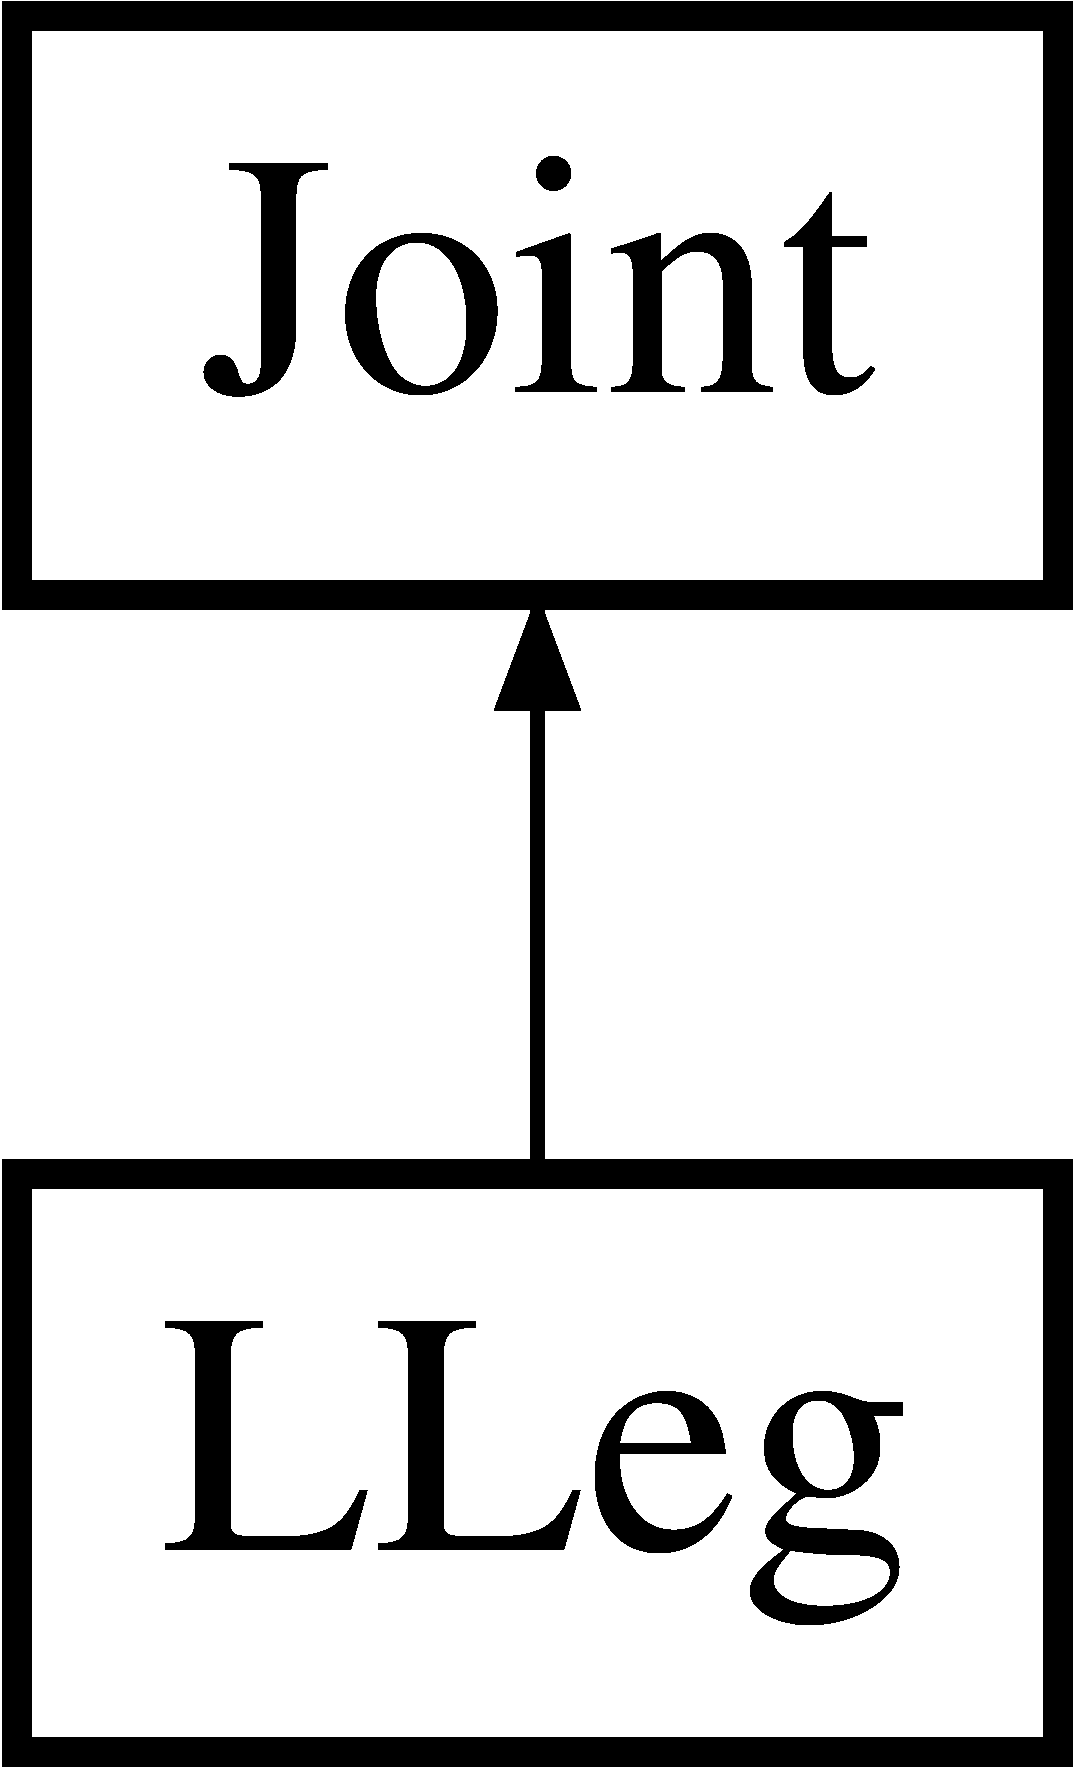
\includegraphics[height=2.000000cm]{class_l_leg}
\end{center}
\end{figure}
\subsection*{Public Member Functions}
\begin{DoxyCompactItemize}
\item 
virtual float \hyperlink{class_l_leg_ac0d2147e72701ad8202b758bb572735f}{get\-Hip\-Roll} (Xn\-User\-I\-D, xn\-::\-User\-Generator)
\begin{DoxyCompactList}\small\item\em Obtiene el angulo que se determina a partir del kinect del hombro. \end{DoxyCompactList}\item 
\hypertarget{class_l_leg_a200afc21f99236f2af57b95ea648573b}{virtual float \hyperlink{class_l_leg_a200afc21f99236f2af57b95ea648573b}{set\-Hip\-Roll} (float, float \&, float \&)}\label{class_l_leg_a200afc21f99236f2af57b95ea648573b}

\begin{DoxyCompactList}\small\item\em Genera el angulo necesario para mover el N\-A\-O. \end{DoxyCompactList}\item 
\hypertarget{class_l_leg_a4a31233e6def8edde81e5d694b7e0feb}{virtual float \hyperlink{class_l_leg_a4a31233e6def8edde81e5d694b7e0feb}{get\-Knee\-Pitch} (Xn\-User\-I\-D, xn\-::\-User\-Generator)}\label{class_l_leg_a4a31233e6def8edde81e5d694b7e0feb}

\begin{DoxyCompactList}\small\item\em Obtiene el angulo que se determina a partir del kinect. \end{DoxyCompactList}\item 
\hypertarget{class_l_leg_a15417e9792bbc9a2f398ed9127e3db11}{virtual float \hyperlink{class_l_leg_a15417e9792bbc9a2f398ed9127e3db11}{set\-Knee\-Pitch} (float, float \&, float \&)}\label{class_l_leg_a15417e9792bbc9a2f398ed9127e3db11}

\begin{DoxyCompactList}\small\item\em Genera el angulo necesario para mover el N\-A\-O. \end{DoxyCompactList}\item 
\hypertarget{class_l_leg_a85ec581c8db5d113a13be644a851753e}{virtual float \hyperlink{class_l_leg_a85ec581c8db5d113a13be644a851753e}{get\-Ankle\-Pitch} (Xn\-User\-I\-D, xn\-::\-User\-Generator)}\label{class_l_leg_a85ec581c8db5d113a13be644a851753e}

\begin{DoxyCompactList}\small\item\em Obtiene el angulo que se determina a partir del kinect. \end{DoxyCompactList}\item 
\hypertarget{class_l_leg_ab474375cb60e68fbf5790459b690b42f}{virtual float \hyperlink{class_l_leg_ab474375cb60e68fbf5790459b690b42f}{set\-Ankle\-Pitch} (float, float \&, float \&)}\label{class_l_leg_ab474375cb60e68fbf5790459b690b42f}

\begin{DoxyCompactList}\small\item\em Genera angulo para mover N\-A\-O. \end{DoxyCompactList}\end{DoxyCompactItemize}


\subsection{Member Function Documentation}
\hypertarget{class_l_leg_ac0d2147e72701ad8202b758bb572735f}{\index{L\-Leg@{L\-Leg}!get\-Hip\-Roll@{get\-Hip\-Roll}}
\index{get\-Hip\-Roll@{get\-Hip\-Roll}!LLeg@{L\-Leg}}
\subsubsection[{get\-Hip\-Roll}]{\setlength{\rightskip}{0pt plus 5cm}float L\-Leg\-::get\-Hip\-Roll (
\begin{DoxyParamCaption}
\item[{Xn\-User\-I\-D}]{user, }
\item[{xn\-::\-User\-Generator}]{guser}
\end{DoxyParamCaption}
)\hspace{0.3cm}{\ttfamily [virtual]}}}\label{class_l_leg_ac0d2147e72701ad8202b758bb572735f}


Obtiene el angulo que se determina a partir del kinect del hombro. 

Obtiene el angulo real dado por el kinect del movimiento del codo. 

The documentation for this class was generated from the following files\-:\begin{DoxyCompactItemize}
\item 
/home/daniel/\-U\-C\-R/\-Ey\-A\-Team/kinect/\-Open\-N\-I\-\_\-\-N\-I\-T\-E\-\_\-\-Installer-\/\-Linux64-\/0.\-27/\-Open\-N\-I-\/\-Bin-\/\-Dev-\/\-Linux-\/x64-\/v1.\-5.\-4.\-0/\-Samples/\-Ni\-Simple\-Skeleton/kinao/joint.\-h\item 
/home/daniel/\-U\-C\-R/\-Ey\-A\-Team/kinect/\-Open\-N\-I\-\_\-\-N\-I\-T\-E\-\_\-\-Installer-\/\-Linux64-\/0.\-27/\-Open\-N\-I-\/\-Bin-\/\-Dev-\/\-Linux-\/x64-\/v1.\-5.\-4.\-0/\-Samples/\-Ni\-Simple\-Skeleton/kinao/lleg.\-cpp\end{DoxyCompactItemize}

\hypertarget{class_r_arm}{\section{{\-R\-Arm \-Class \-Reference} \-R\-Arm}
\label{class_r_arm}\index{\-R\-Arm@{\-R\-Arm}}
}
\-Diagrama de herencia para \-R\-Arm\-:\begin{figure}[H]
\begin{center}
\leavevmode
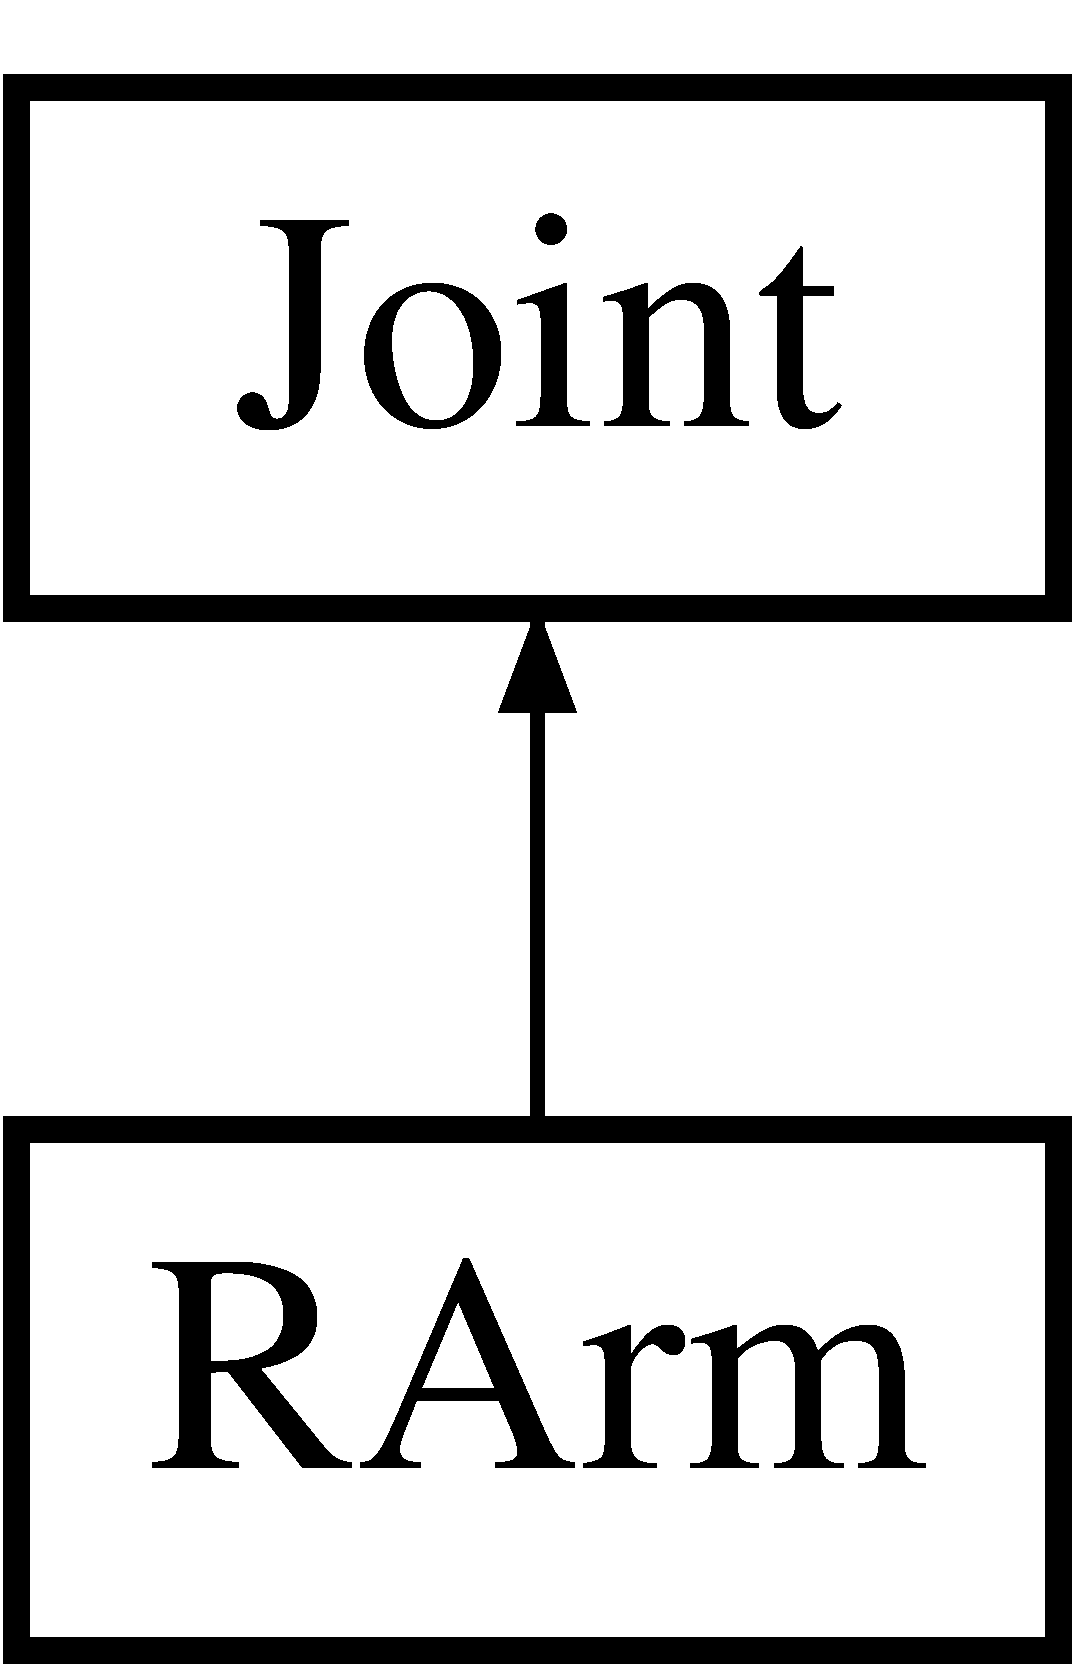
\includegraphics[height=2.000000cm]{class_r_arm}
\end{center}
\end{figure}
\subsection*{\-Public \-Member \-Functions}
\begin{itemize}
\item 
virtual float \hyperlink{class_r_arm_a5c91fecc7fea6e246ce87aac487bde4f}{get\-Elbow\-Roll} (\-Xn\-User\-I\-D, xn\-::\-User\-Generator)
\begin{itemize}\small\item\em \-Obtiene el ángulo que se determina a partir del kinect del codo. \end{itemize}\item 
\hypertarget{class_r_arm_a4788e34770371ab502e1a0d35ec41231}{virtual float \hyperlink{class_r_arm_a4788e34770371ab502e1a0d35ec41231}{set\-Elbow\-Roll} (float, float \&, float \&)}\label{class_r_arm_a4788e34770371ab502e1a0d35ec41231}

\begin{itemize}\small\item\em \-Genera el ángulo al que se necesita mover el \-N\-A\-O. \end{itemize}\item 
\hypertarget{class_r_arm_a273b56a909d68b769dc1ee4aab39fa55}{virtual float \hyperlink{class_r_arm_a273b56a909d68b769dc1ee4aab39fa55}{get\-Shoulder\-Roll} (\-Xn\-User\-I\-D, xn\-::\-User\-Generator)}\label{class_r_arm_a273b56a909d68b769dc1ee4aab39fa55}

\begin{itemize}\small\item\em \-Obtiene el ángulo que se determina a partir del kinect del hombro. \end{itemize}\item 
\hypertarget{class_r_arm_aef1de77829d8fe536eed27639408771b}{virtual float \hyperlink{class_r_arm_aef1de77829d8fe536eed27639408771b}{set\-Shoulder\-Roll} (float, float \&, float \&)}\label{class_r_arm_aef1de77829d8fe536eed27639408771b}

\begin{itemize}\small\item\em \-Genera el ángulo necesario al que se debe mover el \-N\-A\-O. \end{itemize}\item
\hypertarget{class_r_arm_a2647e80238d7767765777fae35ec92bb}{virtual float \hyperlink{class_r_arm_a2647e80238d7767765777fae35ec92bb}{get\-Elbow\-Yaw} (\-Xn\-User\-I\-D, xn\-::\-User\-Generator)}\label{class_r_arm_a2647e80238d7767765777fae35ec92bb}

\item 
\hypertarget{class_r_arm_a72b8946ae53bc1697bdd8371468334ba}{virtual float \hyperlink{class_r_arm_a72b8946ae53bc1697bdd8371468334ba}{set\-Elbow\-Yaw} (float, float \&, float \&)}\label{class_r_arm_a72b8946ae53bc1697bdd8371468334ba}

\end{itemize}

\subsection{\-Descripción \-Detallada}
\-Aquí se describe la clase derivada \char`\"{}\-RArm\char`\"{}. 

\subsection{\-Documentación de \-Función \-Miembro}
\hypertarget{class_r_arm_a5c91fecc7fea6e246ce87aac487bde4f}{\index{\-R\-Arm@{\-R\-Arm}!get\-Elbow\-Roll@{get\-Elbow\-Roll}}
\index{get\-Elbow\-Roll@{get\-Elbow\-Roll}!RArm@{\-R\-Arm}}
\subsubsection[{get\-Elbow\-Roll}]{\setlength{\rightskip}{0pt plus 5cm}float {\bf \-R\-Arm\-::get\-Elbow\-Roll} (
[{\-Xn\-User\-I\-D}]{user, }
[{xn\-::\-User\-Generator}]{guser}
)\hspace{0.3cm}{\ttfamily  \mbox{[}virtual\mbox{]}}}}\label{class_r_arm_a5c91fecc7fea6e246ce87aac487bde4f}


\-Primero se obtienen los puntos que van a determinar el ángulo de codo, se toman los puntos de la muñeca, codo y hombro.\\
\-Luego, utilizando las funciones descritas en la función base Joint, se procede a determinar el ángulo para el movimiento del codo. 

\-La documentación para esta clase fue generada apartir de los archivos\-:\begin{itemize}
\item 
joint.\-h\item 
rarm.\-cpp\end{itemize}

\hypertarget{class_r_leg}{\section{R\-Leg Class Reference}
\label{class_r_leg}\index{R\-Leg@{R\-Leg}}
}
Inheritance diagram for R\-Leg\-:\begin{figure}[H]
\begin{center}
\leavevmode
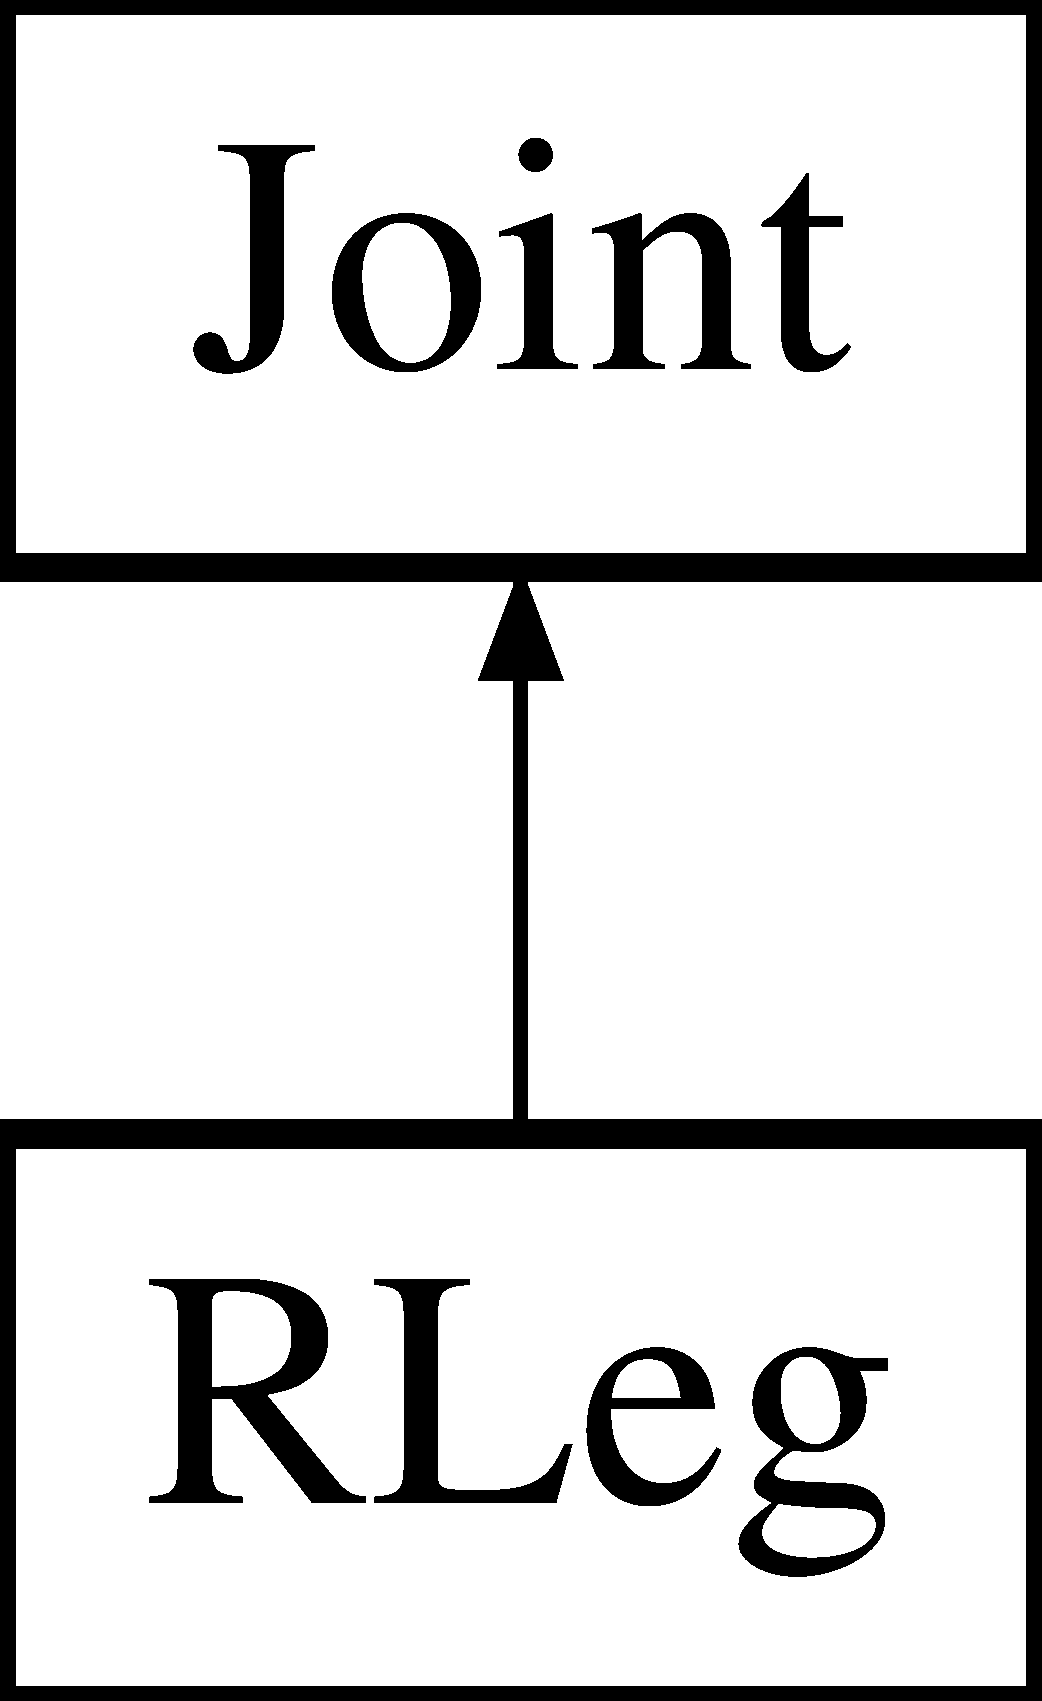
\includegraphics[height=2.000000cm]{class_r_leg}
\end{center}
\end{figure}
\subsection*{Public Member Functions}
\begin{DoxyCompactItemize}
\item 
virtual float \hyperlink{class_r_leg_a983e8da29c577737694dc72a9573fc5c}{get\-Hip\-Roll} (Xn\-User\-I\-D, xn\-::\-User\-Generator)
\begin{DoxyCompactList}\small\item\em Obtiene el angulo que se determina a partir del kinect del hombro. \end{DoxyCompactList}\item 
\hypertarget{class_r_leg_a44386f31cf1afb03ab3f433a0189d820}{virtual float \hyperlink{class_r_leg_a44386f31cf1afb03ab3f433a0189d820}{set\-Hip\-Roll} (float, float \&, float \&)}\label{class_r_leg_a44386f31cf1afb03ab3f433a0189d820}

\begin{DoxyCompactList}\small\item\em Genera el angulo necesario para mover el N\-A\-O. \end{DoxyCompactList}\item 
\hypertarget{class_r_leg_a1e66a29fe07ec16275f86bffe7482fee}{virtual float \hyperlink{class_r_leg_a1e66a29fe07ec16275f86bffe7482fee}{get\-Knee\-Pitch} (Xn\-User\-I\-D, xn\-::\-User\-Generator)}\label{class_r_leg_a1e66a29fe07ec16275f86bffe7482fee}

\begin{DoxyCompactList}\small\item\em Obtiene el angulo que se determina a partir del kinect. \end{DoxyCompactList}\item 
\hypertarget{class_r_leg_a65c0d913ed2c07515cd178b190b4287c}{virtual float \hyperlink{class_r_leg_a65c0d913ed2c07515cd178b190b4287c}{set\-Knee\-Pitch} (float, float \&, float \&)}\label{class_r_leg_a65c0d913ed2c07515cd178b190b4287c}

\begin{DoxyCompactList}\small\item\em Genera el angulo necesario para mover el N\-A\-O. \end{DoxyCompactList}\item 
\hypertarget{class_r_leg_aa8a63cd3f3d06ace1566a531b5213860}{virtual float \hyperlink{class_r_leg_aa8a63cd3f3d06ace1566a531b5213860}{get\-Ankle\-Pitch} (Xn\-User\-I\-D, xn\-::\-User\-Generator)}\label{class_r_leg_aa8a63cd3f3d06ace1566a531b5213860}

\begin{DoxyCompactList}\small\item\em Obtiene el angulo que se determina a partir del kinect. \end{DoxyCompactList}\item 
\hypertarget{class_r_leg_a6ac413efc8dc05dce14096d9797f9149}{virtual float \hyperlink{class_r_leg_a6ac413efc8dc05dce14096d9797f9149}{set\-Ankle\-Pitch} (float, float \&, float \&)}\label{class_r_leg_a6ac413efc8dc05dce14096d9797f9149}

\begin{DoxyCompactList}\small\item\em Genera angulo para mover N\-A\-O. \end{DoxyCompactList}\end{DoxyCompactItemize}


\subsection{Member Function Documentation}
\hypertarget{class_r_leg_a983e8da29c577737694dc72a9573fc5c}{\index{R\-Leg@{R\-Leg}!get\-Hip\-Roll@{get\-Hip\-Roll}}
\index{get\-Hip\-Roll@{get\-Hip\-Roll}!RLeg@{R\-Leg}}
\subsubsection[{get\-Hip\-Roll}]{\setlength{\rightskip}{0pt plus 5cm}float R\-Leg\-::get\-Hip\-Roll (
\begin{DoxyParamCaption}
\item[{Xn\-User\-I\-D}]{user, }
\item[{xn\-::\-User\-Generator}]{guser}
\end{DoxyParamCaption}
)\hspace{0.3cm}{\ttfamily [virtual]}}}\label{class_r_leg_a983e8da29c577737694dc72a9573fc5c}


Obtiene el angulo que se determina a partir del kinect del hombro. 

Obtiene el angulo real dado por el kinect del movimiento del codo. 

The documentation for this class was generated from the following files\-:\begin{DoxyCompactItemize}
\item 
/home/daniel/\-U\-C\-R/\-Ey\-A\-Team/kinect/\-Open\-N\-I\-\_\-\-N\-I\-T\-E\-\_\-\-Installer-\/\-Linux64-\/0.\-27/\-Open\-N\-I-\/\-Bin-\/\-Dev-\/\-Linux-\/x64-\/v1.\-5.\-4.\-0/\-Samples/\-Ni\-Simple\-Skeleton/kinao/joint.\-h\item 
/home/daniel/\-U\-C\-R/\-Ey\-A\-Team/kinect/\-Open\-N\-I\-\_\-\-N\-I\-T\-E\-\_\-\-Installer-\/\-Linux64-\/0.\-27/\-Open\-N\-I-\/\-Bin-\/\-Dev-\/\-Linux-\/x64-\/v1.\-5.\-4.\-0/\-Samples/\-Ni\-Simple\-Skeleton/kinao/rleg.\-cpp\end{DoxyCompactItemize}

\hypertarget{struct_xn_reference_axis}{\section{Xn\-Reference\-Axis Struct Reference}
\label{struct_xn_reference_axis}\index{Xn\-Reference\-Axis@{Xn\-Reference\-Axis}}
}


Definimos un struct \hyperlink{struct_xn_reference_axis}{Xn\-Reference\-Axis} para construir ejes de referencia a partir de vectores.  


\subsection*{Public Attributes}
\begin{DoxyCompactItemize}
\item 
\hypertarget{struct_xn_reference_axis_a4ac206c12a05a55ca3b556525f53c072}{Xn\-Vector3\-D {\bfseries New\-X}}\label{struct_xn_reference_axis_a4ac206c12a05a55ca3b556525f53c072}

\item 
\hypertarget{struct_xn_reference_axis_abe619023a45ec8a7c827f9e42aedf070}{Xn\-Vector3\-D \hyperlink{struct_xn_reference_axis_abe619023a45ec8a7c827f9e42aedf070}{New\-Y}}\label{struct_xn_reference_axis_abe619023a45ec8a7c827f9e42aedf070}

\begin{DoxyCompactList}\small\item\em Es un vector de coordenadas del nuevo eje en X. \end{DoxyCompactList}\item 
\hypertarget{struct_xn_reference_axis_a149a25a6e03ea545d2e99b03a825da51}{Xn\-Vector3\-D \hyperlink{struct_xn_reference_axis_a149a25a6e03ea545d2e99b03a825da51}{New\-Z}}\label{struct_xn_reference_axis_a149a25a6e03ea545d2e99b03a825da51}

\begin{DoxyCompactList}\small\item\em Es un vector de coordenadas del nuevo eje en Y. \end{DoxyCompactList}\end{DoxyCompactItemize}


\subsection{Detailed Description}
Definimos un struct \hyperlink{struct_xn_reference_axis}{Xn\-Reference\-Axis} para construir ejes de referencia a partir de vectores. 

The documentation for this struct was generated from the following files\-:\begin{DoxyCompactItemize}
\item 
/home/daniel/\-U\-C\-R/\-Ey\-A\-Team/kinect/\-Open\-N\-I\-\_\-\-N\-I\-T\-E\-\_\-\-Installer-\/\-Linux64-\/0.\-27/\-Open\-N\-I-\/\-Bin-\/\-Dev-\/\-Linux-\/x64-\/v1.\-5.\-4.\-0/\-Samples/\-Ni\-Simple\-Skeleton/kinao/definition.\-h\item 
/home/daniel/\-U\-C\-R/\-Ey\-A\-Team/kinect/\-Open\-N\-I\-\_\-\-N\-I\-T\-E\-\_\-\-Installer-\/\-Linux64-\/0.\-27/\-Open\-N\-I-\/\-Bin-\/\-Dev-\/\-Linux-\/x64-\/v1.\-5.\-4.\-0/\-Samples/\-Ni\-Simple\-Skeleton/kinao/normal.\-cpp\end{DoxyCompactItemize}

%%%%%%%%%%%%%%%%%%%%%%%%%%%%%%%%%%%%%%%%%%%%%%%%%%%%%%%%%%%%%%%%%%%%%%%%%%%%%%%%%%%%%%%%%%%%%%%%%%%%%%%%%%%%%%%%%

		\begin{figure}[h!]
			\centering
			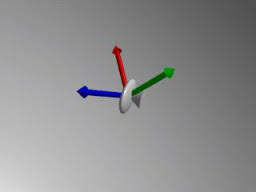
\includegraphics[width=0.55\linewidth]{imagenes/coordenadas-rotado.jpeg}
			\caption{Eje de coordenadas rotado y trasladado en el espacio}
		\end{figure}

%%%%%%%%%%%%%%%%%%%%%%%%%%%%%%%%%%%%%%%%%%%%%%%%%%%%%%%%%%%%%%%%%%%%%%%%%%%%%%%%%%%%%%%%%%%%%%%%%%%%%%%%%%%%%%%%%%
\section{Conclusiones y Recomendaciones}
Se ha analizado las adiciones realizadas al proyecto openni para lograr extraer la información de los ángulos de rotación de brazs y piernas para su posterior conversión a una escala compatible con el NAO. Para ello se agregaron funciones de álgebra lineal compatibles con los tipos de datos de  openni, y además se  agregó una nueva estructura XnReferenceAxis, el cual almacena 3 vectores  correspondientes a un nuevo eje de coordenadas. \\

Ha sido posible concluir que a pesar de las ventajas del Kinect mediante Openni,  pueden llegar a existir ciertas limitaciones en cuanto a documentación (particularmente por el cierre del proyecto openni).\\

Además, existe una limitación a la hora de que la persona que está siendo detectada se coloco de perfil frente al kinect, pues ya el dispositivo no lee directamente la información del otro perfil de la persona, generando datos incompletos o erroneos, o cuando se utiliza ropa holgada, la cual puede  provocar que no se detecten correctamente las rotaciones o torque de forma  adecuada. Otro detalle, el cual  está más directamente relacionado con las funciones agregadas, es la  generaciónd de datos erroneos  en ciertas posiciones, como por ejemplo los brazos completamente extendidos,  en donde algunos de los parámetros  que se emplean  en los cálculos se  indefinen.\\

Dado lo anterior  se recomienda mejorar los algoritmos de detección de rotación para hacerlos más robustos ante estos  detalles, así como ampliar la capacidad de recepción de información, ya sea empleando un segundo dispositivo kinect o Asus Xtion. Además se  recomiendo migrar esta implementación a un sistema más robusto y complejo, como lo es el Motion Capture, para generar datos de forma más confiable y precisa. Es bueno intentar buscar alternativas a openni para  lograr procesar la información obtenida con el kinect.



%%%%%%%%%%%%%%%%%%%%%%%%%%%%%%%%%%%%%%%%%%%%%%%%%%%%%%%%%%%%%%%%%%%%%%%%%%%%%%%%%%%%%%%%%%%%%%%%%%%%%%%%%%%%%%%%%%
\section{Referencias}

\begin{enumerate}
\item Press, W., Teukolsky, W., Vetterling, W., Flannery, B. \textit{Numerical Recipes: The Art of Scietific Computing}, 3ra. Ed. Cambridge University Press, 2007
\item Cormen, T., Leiserson, C., Rivest, R., Stein, C. \textit{Introduction To Algorithms}, 3ra. Ed. MIT Press, 2009
\item Sedgewick, R., Wayne, K. \textit{Algorithms}, 4ta. Ed. Pearson Education, 2011
\item Eckel, B. \textit{Thinking in C++, volume I}, 2da. Ed. Prentice Hall, 2000
\item Referencias web: \begin{itemize}
	\item Librería alternativa para álgebra lineal\url{http://seldon.sourceforge.net/contents.php}
	\item Cálculo vectorial en c++\url{http://stackoverflow.com/questions/13984154/different-methods-for-finding-angle-between-two-vectors}
	\item Documentación del  robot NAO\url{https://community.aldebaran.com/doc/1-14/index.html}
	\item Instalación openni \url{http://igorbarbosa.com/articles/how-to-install-kin-in-linux-mint-12-ubuntu/}
	\item \url{http://blog.jorgeivanmeza.com/2011/12/instalacion-openni-sensor-kinect-y-nite-en-gnulinux-ubuntu-11-10-desde-fuentes/}
	
	\end{itemize}
\end{enumerate}
	
\section{Anexos: Clases implementadas}

\subsection{class\_head}
Aqui se describe la clase derivada "Head", la cual hereda sus propiedades de joint.h.
\lstinputlisting[language=C++]{code/head.cpp}

\subsection{class\_joint}

\lstinputlisting[language=C++]{code/joint.cpp}

\subsection{class\_l\_arm}
\lstinputlisting[language=C++]{code/larm.cpp}
\subsection{class\_l\_leg}
\lstinputlisting[language=C++]{code/lleg.cpp}
\subsection{class\_r\_arm}
\lstinputlisting[language=C++]{code/rarm.cpp}
\subsection{class\_r\_leg}
\lstinputlisting[language=C++]{code/rleg.cpp}
\subsection{struct\_xn\_reference\_axis}
\lstinputlisting[language=C++]{code/definition.h}	
	
\end{document}

